\documentclass[10pt]{amsart}
\usepackage{geometry}                % See geometry.pdf to learn the layout options. There are lots.
\geometry{letterpaper}                   % ... or a4paper or a5paper or ... 
%\geometry{landscape}                % Activate for for rotated page geometry
%\usepackage[parfill]{parskip}    % Activate to begin paragraphs with an empty line rather than an indent
\usepackage{graphicx}
\usepackage{amssymb}
\usepackage{epstopdf}
\DeclareGraphicsRule{.tif}{png}{.png}{`convert #1 `dirname #1`/`basename #1 .tif`.png}

% LUKE'S SETTINGS
% packages
\usepackage{framed}
\usepackage{xcolor}
\usepackage{hanging}
% paragraph
\setlength\parindent{0pt}
\setlength{\parskip}{1em}
% margins
\addtolength{\oddsidemargin}{0.25in}
\addtolength{\topmargin}{-.875in}
\addtolength{\textheight}{3in}
% frame
\definecolor{shadecolor}{rgb}{0.95,0.95,0.95}
% fixed width font (Courier)
\renewcommand{\ttdefault}{pcr}
% column widths with any alignment
\usepackage{array}
\newcolumntype{L}[1]{>{\raggedright\let\newline\\\arraybackslash\hspace{0pt}}p{#1}} % left-top
\newcolumntype{C}[1]{>{\centering\let\newline\\\arraybackslash\hspace{0pt}}p{#1}}   % center-top
\newcolumntype{R}[1]{>{\raggedleft\let\newline\\\arraybackslash\hspace{0pt}}p{#1}}  % right-top
% no extra space after period
\frenchspacing

% Macros file generated by otu_trading_cards.ipynb
\def\sequence{TACGTAGGTGGCAAGCGTTGTCCGGAATTATTGGGCGTAAAGCGCGCGCA
GGCGGTCCTTTAAGTCTGATGTGAAAGCCCACGGCTCAAC}
\def\taxonomyGG{k\_\_Bacteria; p\_\_Firmicutes; c\_\_Bacilli; o\_\_Bacillales; f\_\_Bacillaceae; g\_\_Bacillus; s\_\_foraminis}
\def\taxonomyRDP{d\_\_Bacteria; k\_\_; p\_\_Firmicutes; c\_\_Bacilli; o\_\_Bacillales; f\_\_Bacillaceae 1; g\_\_Bacillus (232/500)}
\def\speciesA{Bacillus sp. (171/500)}
\def\speciesB{Lysinibacillus sp. (51/500)}
\def\speciesC{Planococcus sp. (28/500)}
\def\wikipedia{Did not look up Wikipedia page for Bacillus.}
\def\prevalencePercent{30.70}
\def\prevalenceRank{1}
\def\abundancePercent{0.416}
\def\abundanceRank{16}
\def\numOTUs{155002}
\def\trimLength{90}
\def\numSamples{2000}
\def\rarefactionDepth{5000}


% No page numbers
\thispagestyle{empty}

% Document
\begin{document}

\begin{framed} % alt: shaded

\vspace{-6mm}

\begin{center}

\includegraphics[width=12cm]{emp_logo.pdf}
\end{center}

\begin{hangparas}{5.5em}{0}
\texttt{\sequence{}}
\end{hangparas}

\begin{raggedright}
\begin{hangparas}{2em}{1}
    TAXONOMY:   
    
    \begin{small}
    \begin{tabular}{@{} R{3.5cm} @{ } L{11cm}}
    Greengenes lineage: & \taxonomyGG{} \\
    RDP (100\% ID) lineage: & \taxonomyRDP{} \\
    RDP (100\% ID) species: & \speciesA{} \speciesB{} \speciesC{} \\
    \end{tabular}
	\end{small}

    WIKIPEDIA:  \wikipedia{}

    PREVALENCE: Found in \prevalencePercent{}\% of samples,
                rank \#\prevalenceRank{} out of \numOTUs{} OTUs.

    ABUNDANCE:  Composes \abundancePercent{}\% of observations,
                rank \#\abundanceRank{} out of \numOTUs{} OTUs.
            
    METHODS:    Amplicon PCR with 16S 515f--806rB V4 primers.
                OTU picking with Deblur, trimmed to \trimLength{}~bp.
                Subset of \numSamples{} samples with even distribution across sample types.
                Rarefied to \rarefactionDepth{} observations per sample.

\end{hangparas}

PREVALENCE BY SAMPLE TYPE:

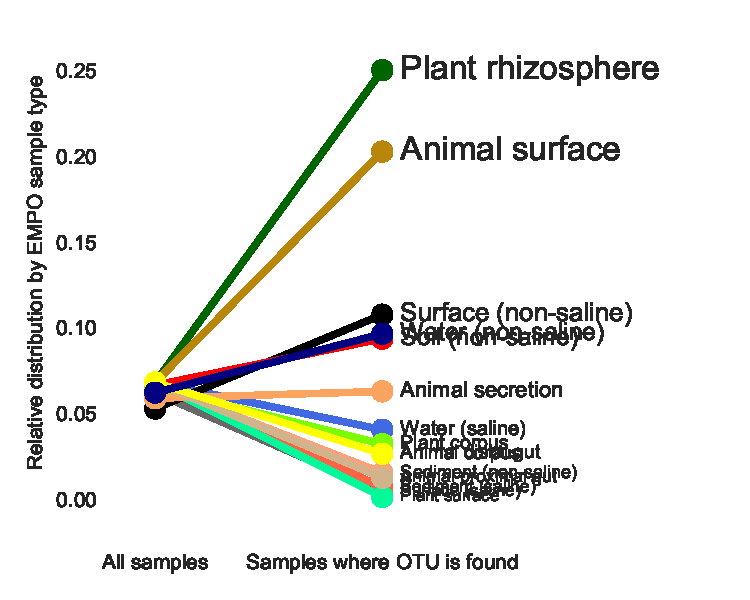
\includegraphics[width=9cm]{point.pdf}

PREVALENCE BY ENVIRONMENTAL PARAMETERS:

\vspace{-3mm}

\begin{center}
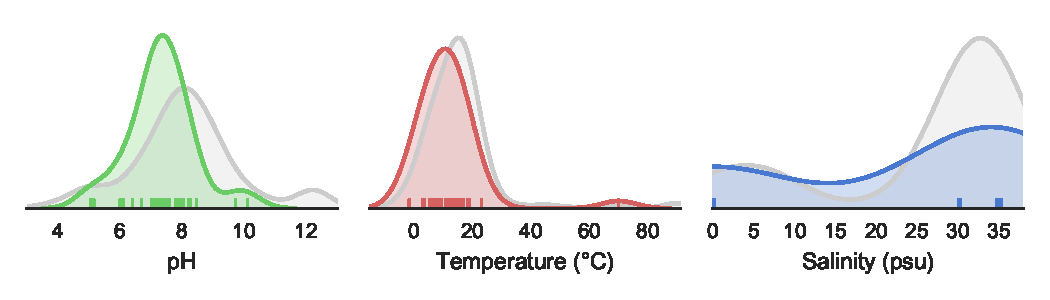
\includegraphics[width=\textwidth]{envparams.pdf}
\end{center}

\end{raggedright}


\begin{center}
    \copyright{} 2016 Earth Microbiome Project
\end{center}

\end{framed}


\end{document}  